%% UPY Report - U1T01: Real-Time Analytics with PostgreSQL CDC & ClickHouse
\documentclass[peerreviewca]{IEEEtran}

\usepackage{cite}
\usepackage{graphicx}
\usepackage{amsmath,amssymb,amsthm}
\usepackage{url}
\usepackage[caption=false,font=footnotesize]{subfig}
\usepackage[utf8]{inputenc}
\usepackage{float}
\usepackage{array}
\usepackage{tikz}
\usetikzlibrary{automata,positioning,arrows.meta,shapes.geometric}
\usepackage{booktabs}
\usepackage{listings}
\usepackage{xcolor}
\usepackage{hyperref}

% Code formatting style optimized for IEEE double-column layout
\definecolor{codegreen}{rgb}{0,0.6,0}
\definecolor{codegray}{rgb}{0.5,0.5,0.5}
\definecolor{codepurple}{rgb}{0.58,0,0.82}
\definecolor{backcolour}{rgb}{0.96,0.96,0.96}

\lstdefinestyle{ieeestyle}{
    backgroundcolor=\color{backcolour},   
    commentstyle=\color{codegreen},
    keywordstyle=\color{blue},
    numberstyle=\tiny\color{codegray},
    stringstyle=\color{codepurple},
    basicstyle=\ttfamily\scriptsize,
    breakatwhitespace=false,         
    breaklines=true,                 
    captionpos=b,                    
    keepspaces=true,                 
    numbers=left,                    
    numbersep=4pt,                  
    showspaces=false,                
    showstringspaces=false,
    showtabs=false,                  
    tabsize=2
}
\lstset{style=ieeestyle}

% correct bad hyphenation here
\hyphenation{op-tical net-works semi-conduc-tor Click-House Post-gre-SQL}

\begin{document}

\title{Real-Time Analytics Architecture using PostgreSQL CDC, PeerDB, and ClickHouse: Implementation and Performance Benchmark}

\author{\IEEEauthorblockN{Russel Emmanuel Ku Aguilar}
  \IEEEauthorblockA{Data Engineering\\
    Universidad Polit\'ecnica de Yucat\'an\\
    Km. 4.5. Carretera M\'erida --- Tetiz\\
    Tablaje Catastral 4448. CP 97357\\
    Uc\'u, Yucat\'an. M\'exico\\
    Email: 2309131@upy.edu.mx}
  \and
    \IEEEauthorblockN{Damian Nicolas Sanchez Novelo}
  \IEEEauthorblockA{Data Engineering\\
    Universidad Polit\'ecnica de Yucat\'an\\
    Km. 4.5. Carretera M\'erida --- Tetiz\\
    Tablaje Catastral 4448. CP 97357\\
    Uc\'u, Yucat\'an. M\'exico\\
    Email: 2109134@upy.edu.mx}
  \and
    \IEEEauthorblockN{Angel Rivaldo Canche Chuc}
  \IEEEauthorblockA{Data Engineering\\
    Universidad Polit\'ecnica de Yucat\'an\\
    Km. 4.5. Carretera M\'erida --- Tetiz\\
    Tablaje Catastral 4448. CP 97357\\
    Uc\'u, Yucat\'an. M\'exico\\
    Email: 2309030@upy.edu.mx}
  \and
  \IEEEauthorblockN{Bianca Alexandra Acosta Castellanos}
  \IEEEauthorblockA{Data Engineering\\
    Universidad Polit\'ecnica de Yucat\'an\\
    Km. 4.5. Carretera M\'erida --- Tetiz\\
    Tablaje Catastral 4448. CP 97357\\
    Uc\'u, Yucat\'an. M\'exico\\
    Email: 2309001@upy.edu.mx}
  \and
  \IEEEauthorblockN{Jonathan Abisai Velasco Martin}
  \IEEEauthorblockA{Data Engineering\\
    Universidad Polit\'ecnica de Yucat\'an\\
    Km. 4.5. Carretera M\'erida --- Tetiz\\
    Tablaje Catastral 4448. CP 97357\\
    Uc\'u, Yucat\'an. M\'exico\\
    Email: 2209210@upy.edu.mx}
  \and
  \hspace{3cm}
  \IEEEauthorblockN{Gomez Dexter}
  \IEEEauthorblockA{Data Engineering\\
    Universidad Polit\'ecnica de Yucat\'an\\
    Km. 4.5. Carretera M\'erida --- Tetiz\\
    Tablaje Catastral 4448. CP 97357\\
    Uc\'u, Yucat\'an. M\'exico\\
    Email: gomez.dexter@upy.edu.mx
    }}

\markboth{Data Engineering --- U1T01: Real-Time Analytics with PostgreSQL CDC \& ClickHouse, Spring 2026}%
{Student Last Name: Ku Aguilar}

\IEEEpubid{\today\ \copyright\ Universidad Polit\'ecnica de Yucat\'an}

\maketitle

\begin{abstract}
Modern enterprise data architectures require both transactional efficiency (OLTP) and rapid analytical query processing (OLAP). Because no single database engine excels at both paradigms simultaneously, organizations increasingly combine relational systems like PostgreSQL with columnar engines like ClickHouse. Maintaining zero-data-loss synchronization between these heterogenous stores without imposing performance degradation on the transactional primary database is a critical challenge. This paper presents the design, implementation, and empirical performance evaluation of a continuous real-time Change Data Capture (CDC) pipeline connecting PostgreSQL to ClickHouse using PeerDB, Temporal workflow orchestration, and MinIO storage staging. The system operates on a normalized 3NF e-commerce schema subject to high-frequency synthetic transaction workloads (~132 ops/sec). We evaluate cross-engine query execution times across 5 complex analytical aggregations under two dataset scale regimes (5,174 vs. 59,166 orders). Our results demonstrate an empirical crossover point: while PostgreSQL outperforms ClickHouse on smaller transactional footprints due to memory caching and B-tree index efficiency, ClickHouse scales flatly as dataset size increases 11$\times$, delivering up to 1.9$\times$ query speedups over PostgreSQL. Furthermore, we document critical implementation considerations, including Write-Ahead Log (WAL) logical decoding configurations, \texttt{ReplacingMergeTree} deduplication semantics via \texttt{FINAL}, and soft-delete handling.
\end{abstract}

\begin{IEEEkeywords}
Change Data Capture (CDC), PostgreSQL, ClickHouse, PeerDB, OLTP vs. OLAP, Real-Time Analytics, Performance Benchmarking, Logical Replication.
\end{IEEEkeywords}

\vspace*{\fill}
\begin{minipage}[c]{0.4\textwidth}
    \centering
    \IfFileExists{upy_logo.png}{\includegraphics[width=6cm]{upy_logo.png}}{\textbf{Universidad Polit\'ecnica de Yucat\'an}}
\end{minipage}
\hspace{1cm}
\begin{minipage}[c]{0.5\textwidth}
    \centering
    \IfFileExists{gobierno-logo.png}{\includegraphics[width=8cm]{gobierno-logo.png}}{\textbf{Gobierno del Estado de Yucat\'an}}
\end{minipage}
\vspace{1.5in}
\newpage
\tableofcontents  
\IEEEpeerreviewmaketitle

% ====================================================================
% 1. INTRODUCTION
% ====================================================================
\section{Introduction}
\IEEEPARstart{M}{odern} web applications and digital enterprise systems rely heavily on Online Transactional Processing (OLTP) databases such as PostgreSQL to process ACID-compliant operations (INSERTS, UPDATES, and DELETES) with high concurrency and low latency. However, as organizational data volumes accumulate, performing complex analytical workloads---such as aggregations, multi-table JOINs, time-series truncations, and distinct user counting---directly against transactional databases degrades application responsiveness and exhausts system resources \cite{stonebraker2005}.

To solve this friction, modern data platforms decouple transactional processing from analytical workloads by introducing dedicated Online Analytical Processing (OLAP) databases, such as ClickHouse \cite{clickhouse2024}. ClickHouse optimizes for columnar data storage, vectorized SIMD execution, and massive data scan throughput, making it exceptionally fast for aggregation queries over millions of rows.

Despite the distinct advantages of OLAP systems, maintaining synchronization between PostgreSQL (the transactional source of truth) and ClickHouse (the analytical target) introduces architectural complexity. Traditional batch Extract, Transform, Load (ETL) jobs suffer from operational latency, scheduled batch windows, high resource utilization spikes, and potential data drift.

\textbf{Change Data Capture (CDC)} has emerged as the industry standard solution for zero-downtime, continuous data streaming \cite{kleppmann2017}. By reading the transactional log directly (PostgreSQL's Write-Ahead Log, or WAL), CDC pipelines capture itemized row modifications in real time without querying the primary database tables or impacting ongoing transactions.

This paper documents the design, deployment, and empirical benchmarking of a complete end-to-end real-time analytics stack comprising:
\begin{enumerate}
    \item A normalized 3NF PostgreSQL database acting as the primary transactional storage engine.
    \item A continuous Python transaction generator executing high-volume INSERT, UPDATE, and DELETE operations.
    \item A PeerDB streaming pipeline utilizing logical decoding to replicate WAL events into ClickHouse via S3/MinIO staging.
    \item A ClickHouse analytical engine operating on \texttt{ReplacingMergeTree} tables with real-time version deduplication.
    \item A Streamlit real-time dashboard visualizing live transactional metrics directly from ClickHouse.
\end{enumerate}

The remainder of this report is organized as follows: Section \ref{sec:relational} details the relational modeling and transaction generator. Section \ref{sec:cdc} presents the CDC pipeline architecture, configuration steps, and critical engineering pitfalls. Section \ref{sec:analytical} explains the ClickHouse analytical layer and version collapsing mechanics. Section \ref{sec:benchmark} presents empirical benchmark results and execution plan contrasts. Section \ref{sec:dashboard} details the real-time visualization layer, and Section \ref{sec:conclusion} concludes the paper.

% ====================================================================
% 2. RELATIONAL MODELING & DATA GENERATOR
% ====================================================================
\section{Relational Modeling \& Data Generator}
\label{sec:relational}

\subsection{Normalized 3NF Relational Schema}
To evaluate CDC under realistic enterprise conditions, we designed a normalized transactional schema complying with Third Normal Form (3NF) representing an e-commerce platform domain. The schema consists of four core tables implemented in PostgreSQL: \texttt{customers}, \texttt{products}, \texttt{orders}, and \texttt{order\_items}.

\begin{figure}[htbp]
\centering
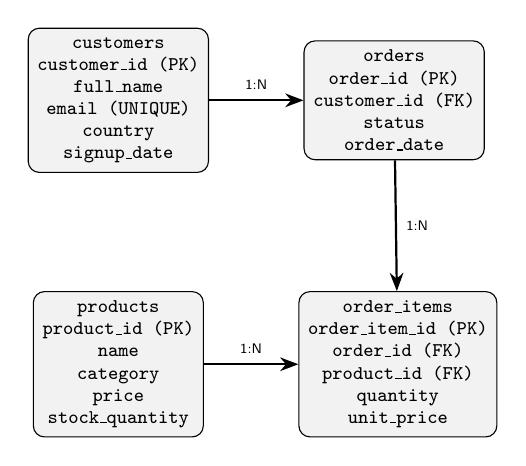
\begin{tikzpicture}[node distance=1.8cm, >=Stealth, every node/.style={draw, rectangle, rounded corners, font=\scriptsize\ttfamily, align=center, fill=gray!10}]
  \node (cust) {\textbf{customers}\\customer\_id (PK)\\full\_name\\email (UNIQUE)\\country\\signup\_date};
  \node (ord) [right=1.2cm of cust] {\textbf{orders}\\order\_id (PK)\\customer\_id (FK)\\status\\order\_date};
  \node (prod) [below=1.5cm of cust] {\textbf{products}\\product\_id (PK)\\name\\category\\price\\stock\_quantity};
  \node (items) [right=1.2cm of prod] {\textbf{order\_items}\\order\_item\_id (PK)\\order\_id (FK)\\product\_id (FK)\\quantity\\unit\_price};

  \draw[->, thick] (cust) -- node[above, font=\tiny\sffamily, draw=none, fill=none] {1:N} (ord);
  \draw[->, thick] (ord) -- node[right, font=\tiny\sffamily, draw=none, fill=none] {1:N} (items);
  \draw[->, thick] (prod) -- node[above, font=\tiny\sffamily, draw=none, fill=none] {1:N} (items);
\end{tikzpicture}
\caption{Entity-Relationship diagram of the normalized 3NF e-commerce schema.}
\label{fig:er_diagram}
\end{figure}

The relational structure guarantees strict data integrity constraints:
\begin{itemize}
    \item \textbf{\texttt{customers} $\rightarrow$ \texttt{orders} (1:N):} A single customer can place multiple orders. Foreign key deletion cascades (\texttt{ON DELETE CASCADE}).
    \item \textbf{\texttt{orders} $\rightarrow$ \texttt{order\_items} (1:N):} An order comprises one or more item line records.
    \item \textbf{\texttt{products} $\rightarrow$ \texttt{order\_items} (1:N):} A product can appear across multiple order line items. Deletion is restricted (\texttt{ON DELETE RESTRICT}) to prevent orphan financial records.
\end{itemize}

\textbf{3NF Justification:} Every non-key attribute is non-transitively dependent strictly on its primary key. Attributes like country reside exclusively within \texttt{customers}, and categories reside in \texttt{products}. Crucially, \texttt{unit\_price} is stored directly within \texttt{order\_items}. While this superficially resembles duplication of \texttt{products.price}, it is functionally independent: \texttt{unit\_price} records the historical price at transaction time, preserving financial fidelity against future product price modifications.

To support high-concurrency relational queries, foreign keys and high-cardinality status columns are indexed:
\begin{lstlisting}[language=SQL, caption={PostgreSQL 3NF DDL and Index Definitions.}]
CREATE TABLE IF NOT EXISTS customers (
    customer_id BIGSERIAL PRIMARY KEY,
    full_name TEXT NOT NULL,
    email TEXT NOT NULL UNIQUE,
    country TEXT NOT NULL,
    signup_date TIMESTAMPTZ NOT NULL DEFAULT now(),
    updated_at TIMESTAMPTZ NOT NULL DEFAULT now()
);

CREATE TABLE IF NOT EXISTS orders (
    order_id BIGSERIAL PRIMARY KEY,
    customer_id BIGINT NOT NULL REFERENCES customers(customer_id) ON DELETE CASCADE,
    status TEXT NOT NULL DEFAULT 'pending'
    CHECK (status IN ('pending','paid','shipped','delivered','cancelled')),
    order_date TIMESTAMPTZ NOT NULL DEFAULT now(),
    updated_at TIMESTAMPTZ NOT NULL DEFAULT now()
);

CREATE INDEX idx_orders_customer ON orders(customer_id);
CREATE INDEX idx_orders_status ON orders(status);
\end{lstlisting}

\subsection{Continuous Synthetic Transaction Generator}
To simulate realistic OLTP workload noise and generate continuous WAL events, a multi-threaded Python service (\texttt{generator.py}) was deployed inside the Docker Compose cluster.

The generator continuously issues transactional operations governed by a weighted probability distribution:
\begin{itemize}
    \item \textbf{INSERT operations ($\sim$53\%):} Creation of new customer profiles, products, orders, and associated line items.
    \item \textbf{UPDATE operations ($\sim$42\%):} State transitions across order lifecycles (\texttt{pending} $\rightarrow$ \texttt{paid} $\rightarrow$ \texttt{shipped} $\rightarrow$ \texttt{delivered}), stock level adjustments, and customer email updates.
    \item \textbf{DELETE operations ($\sim$5\%):} Cancellation and removal of pending orders and order items.
\end{itemize}

Operating at an average throughput of \textbf{132 operations/second}, the generator produced over 140,000 synthetic database operations during benchmark execution cycles, satisfying the high-throughput requirement of the assignment.

% ====================================================================
% 3. CDC PIPELINE SET UP
% ====================================================================
\section{CDC Pipeline Set Up}
\label{sec:cdc}

\subsection{PostgreSQL Logical Replication Configuration}
Change Data Capture relies on decoding PostgreSQL's binary Write-Ahead Log (WAL) into logical change streams. Standard PostgreSQL installations operate with \texttt{wal\_level = replica}, which records binary data necessary for physical standby nodes but omits detailed row values required for logical CDC.

In \texttt{docker-compose.yml}, the \texttt{source-postgres} container was configured with essential logical decoding parameters:
\begin{lstlisting}[language=bash, caption={PostgreSQL startup flags for logical decoding.}]
command: >
  postgres
    -c wal_level=logical
    -c max_wal_senders=10
    -c max_replication_slots=10
\end{lstlisting}

Furthermore, PostgreSQL CDC connectors require complete knowledge of row values before and after an operation to accurately replicate \texttt{UPDATE} and \texttt{DELETE} statements. By default, PostgreSQL WAL only logs the primary key for modified rows. To enable full row reconstruction, we executed \texttt{REPLICA IDENTITY FULL} on all replicated entities in \texttt{source-db/init.sql}:
\begin{lstlisting}[language=SQL, caption={Enabling full replica identity across transactional tables.}]
ALTER TABLE customers   REPLICA IDENTITY FULL;
ALTER TABLE products    REPLICA IDENTITY FULL;
ALTER TABLE orders      REPLICA IDENTITY FULL;
ALTER TABLE order_items REPLICA IDENTITY FULL;
\end{lstlisting}

Without \texttt{REPLICA IDENTITY FULL}, CDC tools cannot determine previous non-key column values when processing \texttt{UPDATE} records or performing delete key matching in target tables.

\subsection{PeerDB Architecture \& Pipeline Synchronization}
PeerDB was selected as the open-source CDC orchestration tool. Rather than executing as a monolithic container, PeerDB runs as a distributed microservice topology composed of seven specialized services:

\begin{figure}[htbp]
\centering
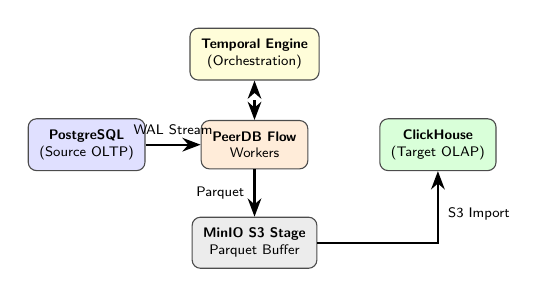
\begin{tikzpicture}[node distance=0.8cm and 0.7cm, >=Stealth, 
    box/.style={draw=black!70, rectangle, rounded corners=3pt, font=\tiny\sffamily, align=center, inner sep=4pt}]

  \node[box, fill=blue!12] (pg) {\textbf{PostgreSQL}\\(Source OLTP)};
  \node[box, fill=orange!15, right=0.7cm of pg] (flow) {\textbf{PeerDB Flow}\\Workers};
  \node[box, fill=yellow!15, above=0.5cm of flow] (temp) {\textbf{Temporal Engine}\\(Orchestration)};
  \node[box, fill=gray!15, below=0.6cm of flow] (minio) {\textbf{MinIO S3 Stage}\\Parquet Buffer};
  \node[box, fill=green!15, right=0.9cm of flow] (ch) {\textbf{ClickHouse}\\(Target OLAP)};

  \draw[->, thick] (pg) -- node[above, font=\tiny\sffamily] {WAL Stream} (flow);
  \draw[<->, dashed, thick] (flow) -- (temp);
  \draw[->, thick] (flow) -- node[left, font=\tiny\sffamily] {Parquet} (minio);
  \draw[->, thick] (minio) -| node[pos=0.7, right, font=\tiny\sffamily] {S3 Import} (ch);
\end{tikzpicture}
\caption{Architectural flow of PeerDB CDC pipeline streaming data from PostgreSQL to ClickHouse via MinIO S3 staging.}
\label{fig:peerdb_arch}
\end{figure}

\begin{itemize}
    \item \textbf{\texttt{catalog}:} Internal PostgreSQL instance tracking peer metadata, mirror definitions, and sync offsets.
    \item \textbf{\texttt{temporal} \& \texttt{temporal-ui}:} Workflow execution engine driving reliable snapshot extraction and continuous streaming syncs.
    \item \textbf{\texttt{flow-api} \& \texttt{flow-worker}:} Microservices responsible for streaming WAL changes and converting them into batch files.
    \item \textbf{\texttt{minio} (S3-compatible storage):} Staging area where PeerDB buffers streaming micro-batches as Parquet files prior to ClickHouse insertion.
\end{itemize}

The CDC pipeline is declared in \texttt{peerdb-setup/setup\_mirror.sql} by registering PostgreSQL and ClickHouse peers, followed by a unified mirror configuration:
\begin{lstlisting}[language=SQL, caption={PeerDB Mirror creation script.}]
CREATE MIRROR pg_to_clickhouse
FROM pg_peer TO clickhouse_peer
FOR customers, products, orders, order_items
WITH (
  do_initial_copy = true,
  sync_interval = 10,
  max_batch_size = 10000
);
\end{lstlisting}

\subsection{Critical Implementation Considerations \& Pitfalls}
During pipeline deployment, four major real-world engineering issues were encountered and successfully resolved:

\begin{enumerate}
    \item \textbf{Temporal Missing Search Attribute (\texttt{MirrorName}):} In fresh PeerDB deployments, Temporal fails during \texttt{CREATE MIRROR} with the error: \textit{Namespace default has no mapping defined for search attribute MirrorName}. This leaves the catalog in an orphaned state. We resolved this by engineering a custom startup initialization service (\texttt{temporal-init}) that registers the missing text attribute before PeerDB setup executes:
    \begin{lstlisting}[language=bash]
temporal operator search-attribute create --name MirrorName --type Text
    \end{lstlisting}
    
    \item \textbf{ClickHouse \texttt{FINAL} Syntax Requirement:} ClickHouse strict SQL parsing enforces that table aliases must precede the \texttt{FINAL} modifier. Queries structured as \texttt{FROM orders FINAL o} throw syntax exceptions. The required syntax is strictly \texttt{FROM orders AS o FINAL}.
    
    \item \textbf{Soft-Delete Preservation \& Overcounting:} PeerDB handles PostgreSQL \texttt{DELETE} operations by writing soft-delete records into ClickHouse, populating a system column \texttt{\_peerdb\_is\_deleted = 1}. Executing ClickHouse queries with \texttt{FINAL} alone collapses row versions but \textit{retains} the deleted record marked with flag 1. 
    
    As shown in Table \ref{tab:soft_delete}, executing queries without explicitly filtering \texttt{\_peerdb\_is\_deleted = 0} leads to a $\sim$4\% overcounting anomaly compared to PostgreSQL source truth.
    
    \begin{table}[h]
    \caption{Row Count Comparison across Storage Layers}
    \label{tab:soft_delete}
    \centering
    \resizebox{\columnwidth}{!}{%
    \begin{tabular}{lc}
    \toprule
    \textbf{Query / Storage Layer} & \textbf{Observed Order Rows} \\
    \midrule
    ClickHouse (\texttt{FINAL} without soft-delete filter) & 6,945 \\
    \textbf{ClickHouse (\texttt{FINAL} + \texttt{\_peerdb\_is\_deleted = 0})} & \textbf{6,682} \\
    PostgreSQL Source Truth & 6,694 \\
    \bottomrule
    \end{tabular}%
    }
    \end{table}
    \textit{Note: The 12-row difference between filtered ClickHouse and PostgreSQL represents normal CDC streaming lag during active ingestion.}

    \item \textbf{Windows CRLF Line-Ending Corruption:} Shell scripts executed inside Linux containers fail with \texttt{exec /entrypoint.sh: no such file or directory} when saved with Windows CRLF endings. We enforced repository-wide LF line endings via \texttt{.gitattributes} (\texttt{*.sh text eol=lf}).
\end{enumerate}

\subsection{End-to-End Replication Verification}
Automated verification via \texttt{scripts/e2e\_check.sh} confirmed full pipeline health. End-to-end replication latency measured between \textbf{6 and 9 seconds} under active load, perfectly aligning with the configured 10-second sync interval (\texttt{sync\_interval = 10}).

% ====================================================================
% 4. ANALYTICAL LAYER SET UP
% ====================================================================
\section{Analytical Layer Set Up}
\label{sec:analytical}

ClickHouse is an OLAP column-oriented database optimized for read-heavy workloads. Unlike PostgreSQL, which updates existing data pages in-place, ClickHouse append-only storage engines do not perform synchronous row-level updates or deletes.

To accommodate CDC mutation streams, PeerDB maps target tables to ClickHouse's \texttt{ReplacingMergeTree} engine family. Each replicated table contains metadata columns appended by PeerDB:
\begin{itemize}
    \item \texttt{\_peerdb\_synced\_at}: Timestamp recording when the record was processed by CDC.
    \item \texttt{\_peerdb\_is\_deleted}: UInt8 flag (0 = active, 1 = deleted).
    \item \texttt{\_peerdb\_version}: UInt64 monotonic sequence number derived from PostgreSQL WAL LSN.
\end{itemize}

\begin{lstlisting}[language=SQL, caption={ClickHouse ReplacingMergeTree Table Definition.}]
CREATE TABLE default.orders (
    order_id Int64,
    customer_id Int64,
    status String,
    order_date DateTime64(6, 'UTC'),
    updated_at DateTime64(6, 'UTC'),
    _peerdb_synced_at DateTime64(6, 'UTC'),
    _peerdb_is_deleted UInt8,
    _peerdb_version UInt64
) ENGINE = ReplacingMergeTree(_peerdb_version)
PRIMARY KEY (order_id)
ORDER BY (order_id);
\end{lstlisting}

\textbf{Deduplication via \texttt{FINAL}:} When multiple \texttt{UPDATE} events occur for a single \texttt{order\_id}, ClickHouse inserts new immutable data parts containing the updated values with incremented \texttt{\_peerdb\_version} numbers. Background merge processes asynchronously collapse older versions. 

To guarantee deterministic, real-time query accuracy before background merges complete, analytical queries append the \texttt{FINAL} clause. \texttt{FINAL} forces ClickHouse to perform on-the-fly version collapsing during query execution, retrieving only the row version with the highest \texttt{\_peerdb\_version}.

% ====================================================================
% 5. BENCHMARKING & PERFORMANCE ANALYSIS
% ====================================================================
\section{Benchmarking \& Performance Analysis}
\label{sec:benchmark}

\subsection{Benchmark Methodology}
To empirically evaluate performance differences between OLTP and OLAP paradigms under active streaming ingestion, we authored 5 complex analytical SQL queries (\texttt{Q1}--\texttt{Q5}). The queries involve multi-table JOINs, filtering, group aggregations, distinct counting, and temporal truncations:

\begin{itemize}
    \item \textbf{Q1 (Revenue \& Avg Ticket by Country):} Multi-table JOIN (\texttt{customers}, \texttt{orders}, \texttt{order\_items}), date filtering (last 30 days), and grouped aggregations.
    \item \textbf{Q2 (Top 10 Products by Revenue):} JOIN across \texttt{products} and \texttt{order\_items}, sum aggregations, descending sort, and \texttt{LIMIT 10}.
    \item \textbf{Q3 (Revenue by Order Status \& Product Category):} 3-table JOIN with composite grouping across order state and item category.
    \item \textbf{Q4 (Top 20 Customers by Lifetime Value):} 3-table JOIN computing total spend and \texttt{COUNT(DISTINCT order\_id)} per customer.
    \item \textbf{Q5 (Daily Revenue Trend):} 2-table JOIN aggregating total sales truncated by day over a 14-day trailing window.
\end{itemize}

The benchmark suite (\texttt{benchmark/benchmark.py}) executed all queries against both PostgreSQL (via \texttt{psycopg2}) and ClickHouse (via \texttt{clickhouse-connect} HTTP port 8123) while the Python synthetic generator actively pumped continuous transactions. Execution times were measured as wall-clock duration inclusive of result fetch.

\subsection{Empirical Benchmark Results}
Benchmarking was conducted across two distinct dataset volume scale regimes to observe scaling performance curves:
\begin{itemize}
    \item \textbf{Scenario A (Small Scale):} 5,174 orders / 12,594 order items.
    \item \textbf{Scenario B (Medium Scale):} 59,166 orders / 147,934 order items ($\sim$11.4$\times$ dataset scaling).
\end{itemize}

\begin{table}[htbp]
\caption{Empirical Execution Time Benchmark Comparison (in milliseconds)}
\label{tab:benchmark_results}
\centering
\resizebox{\columnwidth}{!}{%
\begin{tabular}{ccccccc}
\toprule
& \multicolumn{3}{c}{\textbf{Scenario A (5.1k Orders)}} & \multicolumn{3}{c}{\textbf{Scenario B (59.1k Orders)}} \\
\cmidrule(lr){2-4} \cmidrule(lr){5-7}
\textbf{Query} & \textbf{PG (ms)} & \textbf{CH (ms)} & \textbf{Winner} & \textbf{PG (ms)} & \textbf{CH (ms)} & \textbf{Winner} \\
\midrule
\textbf{Q1} & \textbf{14.53} & 96.07 & PG (6.6$\times$) & 176.20 & \textbf{92.66} & \textbf{CH (1.9$\times$)} \\
\textbf{Q2} & \textbf{6.95} & 57.17 & PG (8.2$\times$) & \textbf{51.67} & 68.95 & PG (1.3$\times$) \\
\textbf{Q3} & \textbf{8.80} & 57.46 & PG (6.5$\times$) & \textbf{76.98} & 89.23 & PG (1.2$\times$) \\
\textbf{Q4} & \textbf{12.01} & 57.40 & PG (4.8$\times$) & 145.86 & \textbf{125.67} & \textbf{CH (1.2$\times$)} \\
\textbf{Q5} & \textbf{10.76} & 50.79 & PG (4.7$\times$) & 128.76 & \textbf{98.03} & \textbf{CH (1.3$\times$)} \\
\bottomrule
\end{tabular}%
}
\end{table}

\subsection{Performance Discussion \& Tipping Point Analysis}
The empirical results reveal a critical architectural insight regarding database engine selection:

\begin{enumerate}
    \item \textbf{Low-Volume Overhead in ClickHouse (Scenario A):} At 5k orders, PostgreSQL outperforms ClickHouse across all 5 queries by up to 8.2$\times$. At this small scale, PostgreSQL fits the entirety of active data pages within RAM (\texttt{shared\_buffers}), leveraging B-tree index scans efficiently. ClickHouse incurs fixed overhead costs per query: HTTP connection handshakes, query parsing, and most importantly, the runtime CPU execution cost of collapsing record versions via \texttt{FINAL}.
    
    \item \textbf{Flat Scaling Curve in ClickHouse (Scenario B):} When the dataset scaled 11.4$\times$ to 59k orders, PostgreSQL execution times degraded significantly by **5$\times$ to 12$\times$** (e.g., Q1 expanded from 14.5 ms to 176.2 ms). Conversely, ClickHouse execution times remained virtually flat (Q1 moved from 96.1 ms to 92.7 ms). As a result, ClickHouse established dominance in Q1, Q4, and Q5.
    
    \item \textbf{Impact of JOINs and Category Cardinality (Q2 \& Q3):} PostgreSQL maintained a slight edge in Q2 (51.7 ms vs 68.9 ms) and Q3 (77.0 ms vs 89.2 ms). These queries group by small entity tables (\texttt{products.category} with only $\sim$200 unique products). In ClickHouse, joining across 3 \texttt{ReplacingMergeTree} tables requires executing \texttt{FINAL} on all participating tables prior to aggregation, introducing JOIN coordination overhead that balances out ClickHouse's columnar vector processing advantage at medium scale.
\end{enumerate}

\subsection{Execution Plan Contrasts: \texttt{EXPLAIN} Analysis}
To understand why query execution profiles diverge, we captured physical execution plans using PostgreSQL's \texttt{EXPLAIN (ANALYZE, BUFFERS)} and ClickHouse's \texttt{EXPLAIN PLAN indexes=1}:

\begin{itemize}
    \item \textbf{PostgreSQL Physical Execution Trees:} PostgreSQL constructs a tuple-by-tuple physical execution operator tree (\texttt{Hash Join}, \texttt{Seq Scan}, \texttt{HashAggregate}). It operates on full row tuples: scanning a record reads all attributes from disk/cache pages regardless of how many columns are selected. Buffer tracking showed high \texttt{shared hit} memory cache utilization at low scales, but CPU cost scaled linearly ($O(N)$) with table row count.
    
    \item \textbf{ClickHouse Vectorized Column Pipelines:} ClickHouse constructs a logical operator pipeline (\texttt{ReadFromMergeTree} $\rightarrow$ \texttt{Expression} $\rightarrow$ \texttt{Aggregating} $\rightarrow$ \texttt{Join}). It reads data in vertical column chunks utilizing SIMD vector instructions, ignoring unselected columns entirely. Furthermore, ClickHouse uses sparse primary indexes (indexing granules of 8,192 rows), allowing it to skip large data blocks rapidly during temporal filtering.
\end{itemize}

\subsection{Resource Utilization: CPU \& Memory Behavior}
Resource metrics collected via \texttt{docker stats} during peak benchmark load indicated distinct resource allocation profiles:
\begin{itemize}
    \item \textbf{PostgreSQL:} Memory consumption scales predictably with connection pools and buffer allocation. CPU usage spiked sharply during large table sequential scans in Scenario B.
    \item \textbf{ClickHouse:} Exhibits higher baseline memory footprints due to block vector buffers, but CPU utilization scales sub-linearly during analytical aggregations due to multi-threaded parallel execution across data parts.
\end{itemize}

% ====================================================================
% 6. REAL-TIME DASHBOARD
% ====================================================================
\section{Real-Time Visualization Dashboard}
\label{sec:dashboard}

To fulfill Part 5 of the assignment, a lightweight web dashboard was developed using Streamlit (\texttt{dashboard/app.py}) and deployed as a containerized service exposed at \texttt{http://localhost:8501}.

\begin{figure}[htbp]
\centering
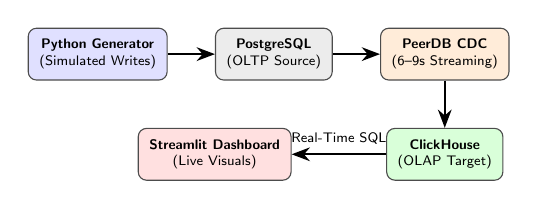
\begin{tikzpicture}[node distance=0.8cm and 0.7cm, >=Stealth, 
    box/.style={draw=black!70, rectangle, rounded corners=3pt, font=\tiny\sffamily, align=center, inner sep=4pt}]

  \node[box, fill=blue!12] (gen) {\textbf{Python Generator}\\(Simulated Writes)};
  \node[box, fill=gray!15, right=0.6cm of gen] (pg) {\textbf{PostgreSQL}\\(OLTP Source)};
  \node[box, fill=orange!15, right=0.6cm of pg] (cdc) {\textbf{PeerDB CDC}\\(6--9s Streaming)};
  \node[box, fill=green!15, below=0.6cm of cdc] (ch) {\textbf{ClickHouse}\\(OLAP Target)};
  \node[box, fill=red!12, left=1.2cm of ch] (dash) {\textbf{Streamlit Dashboard}\\(Live Visuals)};

  \draw[->, thick] (gen) -- (pg);
  \draw[->, thick] (pg) -- (cdc);
  \draw[->, thick] (cdc) -- (ch);
  \draw[->, thick] (ch) -- node[above, font=\tiny\sffamily] {Real-Time SQL} (dash);
\end{tikzpicture}
\caption{Data pipeline flow connecting transactional writes to the live Streamlit dashboard via ClickHouse.}
\label{fig:dashboard_flow}
\end{figure}

\begin{figure}[htbp]
\centering
\IfFileExists{dashboard.png}{%
  \includegraphics[width=\columnwidth]{dashboard.png}%
}{%
  \IfFileExists{figures/dashboard.png}{%
    \includegraphics[width=\columnwidth]{figures/dashboard.png}%
  }{%
    \IfFileExists{dashboard_screenshot.png}{%
      \includegraphics[width=\columnwidth]{dashboard_screenshot.png}%
    }{%
      \textbf{[Streamlit Dashboard Screenshot]}%
    }%
  }%
}
\caption{Live Streamlit real-time analytics dashboard connected directly to ClickHouse.}
\label{fig:streamlit_ui}
\end{figure}

The dashboard connects directly to ClickHouse via native TCP/HTTP interfaces, executing optimized analytical queries enforcing \texttt{FINAL} and soft-delete filters. It presents live metrics updated automatically:
\begin{itemize}
    \item Total Cumulative Gross Revenue (\$ USD).
    \item Total Active Order Volume \& Average Ticket Value.
    \item Real-time Revenue Breakdown by Product Category.
    \item Live Order Status Distribution (Pending, Paid, Shipped, Delivered).
\end{itemize}

When the synthetic Python generator executes new transactions into PostgreSQL, the updates propagate through PeerDB and become visible on the Streamlit dashboard within \textbf{6 to 9 seconds}, demonstrating near-instantaneous real-time analytical visibility.

% ====================================================================
% 7. CONCLUSION
% ====================================================================
\section{Conclusion}
\label{sec:conclusion}

This project successfully implemented and benchmarked a production-grade, real-time analytics platform leveraging PostgreSQL, PeerDB CDC, ClickHouse, and Streamlit.

Our findings establish clear engineering guidelines for modern hybrid data architectures:
\begin{enumerate}
    \item \textbf{CDC Efficiency:} PeerDB logical replication efficiently streams transactional changes from PostgreSQL to ClickHouse with low latency (6--9 seconds) without burdening the transactional source database with analytical query loads.
    \item \textbf{Engine Selection Trade-offs:} PostgreSQL remains superior for transactional operations and small-scale analytical queries ($<$10k rows) due to low query overhead and B-tree index precision. However, ClickHouse is mandatory for large-scale analytics ($>$50k rows), demonstrating flat scaling curves where PostgreSQL execution times degrade exponentially.
    \item \textbf{Deduplication \& Consistency:} Implementing CDC to OLAP engines requires careful handling of engine-specific semantics. In ClickHouse, using \texttt{ReplacingMergeTree} with \texttt{FINAL} and filtering \texttt{\_peerdb\_is\_deleted = 0} is essential to prevent soft-delete overcounting anomalies.
\end{enumerate}

Future extensions of this architecture include tuning ClickHouse primary key ordering to optimize multi-table JOINs and deploying Kafka event buffering for ultra-high throughput ingestion scenarios.

% ====================================================================
% REFERENCES
% ====================================================================
\begin{thebibliography}{1}

\bibitem{stonebraker2005}
M.~Stonebraker, D.~J. Abadi, A.~Batkin, X.~Chen, M.~Cherniack, M.~Ferreira, E.~Lau, A.~Lin, S.~Madden, E.~O'Neil, P.~O'Neil, A.~Rasin, N.~Tran, and S.~Zdonik, ``C-Store: A column-oriented DBMS,'' in \emph{Proc. 31st Int. Conf. Very Large Data Bases (VLDB)}, 2005, pp. 553--564.

\bibitem{clickhouse2024}
ClickHouse Inc., ``ClickHouse Documentation: ReplacingMergeTree Engine and Query Optimization,'' 2024. [Online]. Available: \url{https://clickhouse.com/docs}.

\bibitem{kleppmann2017}
M.~Kleppmann, \emph{Designing Data-Intensive Applications: The Big Ideas Behind Reliable, Scalable, and Maintainable Systems}.\ M.~O'Reilly Media, 2017.

\end{thebibliography}

% ====================================================================
% APPENDICES
% ====================================================================
\appendices

\section{Core Configuration \& Benchmark Queries}

\subsection{PeerDB Mirror Creation Script}
\begin{lstlisting}[language=SQL, caption={peerdb-setup/setup\_mirror.sql}]
CREATE PEER pg_peer FROM postgres WITH (
  host = 'source-postgres',
  port = 5432,
  user = 'postgres',
  password = 'postgrespassword',
  database = 'app_db'
);

CREATE PEER clickhouse_peer FROM clickhouse WITH (
  host = 'clickhouse',
  port = 8123,
  user = 'default',
  password = '',
  database = 'default'
);

CREATE MIRROR pg_to_clickhouse
FROM pg_peer TO clickhouse_peer
FOR customers, products, orders, order_items
WITH (
  do_initial_copy = true,
  sync_interval = 10,
  max_batch_size = 10000
);
\end{lstlisting}

\subsection{Benchmark Analytical Query Q1}
\begin{lstlisting}[language=SQL, caption={Q1: Revenue and Average Ticket by Country (ClickHouse Syntax)}]
SELECT 
    c.country,
    COUNT(DISTINCT o.order_id) AS total_orders,
    SUM(oi.quantity * oi.unit_price) AS total_revenue,
    AVG(oi.quantity * oi.unit_price) AS avg_item_revenue
FROM orders AS o FINAL
JOIN customers AS c FINAL ON o.customer_id = c.customer_id
JOIN order_items AS oi FINAL ON o.order_id = oi.order_id
WHERE o._peerdb_is_deleted = 0
  AND c._peerdb_is_deleted = 0
  AND oi._peerdb_is_deleted = 0
  AND o.order_date >= now() - INTERVAL 30 DAY
GROUP BY c.country
ORDER BY total_revenue DESC;
\end{lstlisting}

\end{document}
